\documentclass[11pt]{article}
\usepackage[textwidth=18.0cm, textheight=23.0cm, top=2.0cm]{geometry}
\usepackage{pst-all}
\usepackage{amssymb}
\usepackage{tikz}
\usepackage{underscore}\begin{document}
\pagestyle{empty}


ClassName: \underline{\textbf{Class_03.2bp-26}}
\par
BinSize: \underline{\textbf{40 × 40}}
\par
ReduceSize: \underline{\textbf{40 × 40}}
\par
TypeNum: \underline{\textbf{59}}
\par
Num: \underline{\textbf{60}}
\par
OutS: \underline{\textbf{17600}}
\par
InS: \underline{\textbf{15937}}
\par
Rate: \underline{\textbf{0.906}}
\par
UB: \underline{\textbf{11}}
\par
LB0: \underline{\textbf{11}}
\par
LB: \underline{\textbf{11}}
\par
LBWithCut: \underline{\textbf{11}}
\par
NodeCut: \underline{\textbf{0}}
\par
ExtendedNodeCnt: \underline{\textbf{1}}
\par
GenNodeCnt: \underline{\textbf{1}}
\par
PrimalNode: \underline{\textbf{0}}
\par
ColumnCount: \underline{\textbf{11}}
\par
TotalCutCount: \underline{\textbf{0}}
\par
RootCutCount: \underline{\textbf{0}}
\par
LPSolverCnt: \underline{\textbf{1}}
\par
PricingSolverCnt: \underline{\textbf{0}}
\par
BranchAndBoundNum: \underline{\textbf{1}}
\par
isOpt: \underline{\textbf{true}}
\par
TimeOnPrimal: \underline{\textbf{0.000 s}}
\par
TimeOnPricing: \underline{\textbf{0.000 s}}
\par
TimeOnRmp: \underline{\textbf{0.078 s}}
\par
TotalTime: \underline{\textbf{0.141 s}}
\par
\newpage


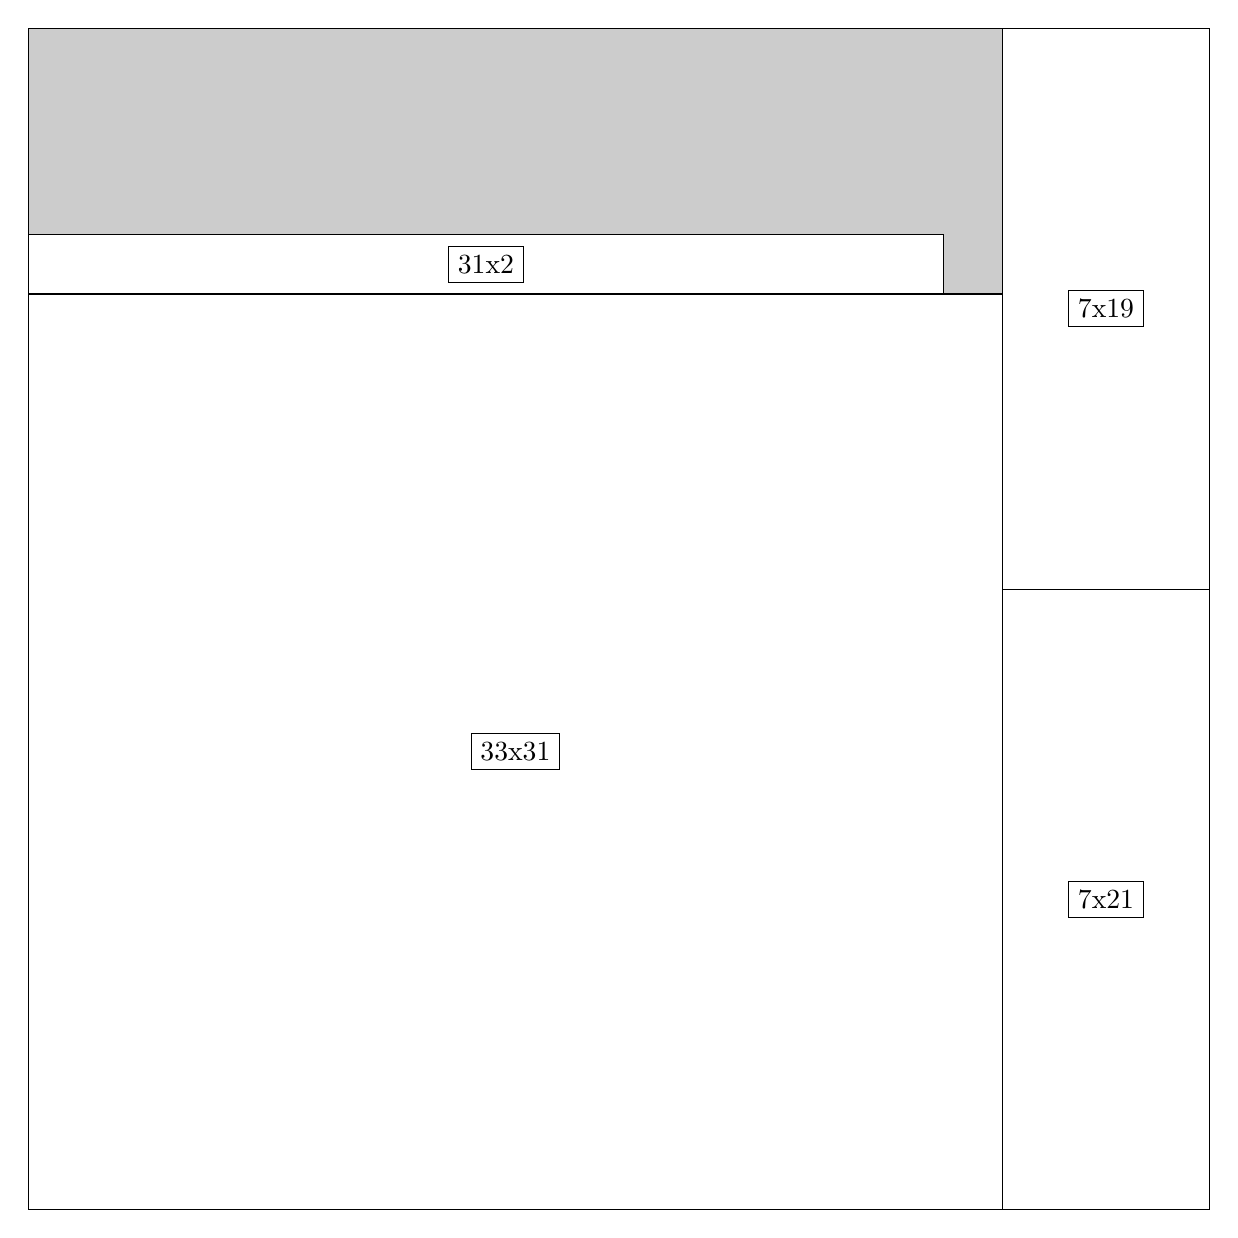
\begin{tikzpicture}[shorten >=1pt,scale=1.0,every node/.style={scale=1.0},->]
\tikzstyle{vertex}=[circle,fill=black!25,minimum size=14pt,inner sep=0pt]
\filldraw[fill=gray!40!white, draw=black] (0,0) rectangle (15.0,15.0);
\foreach \name/\x/\y/\w/\h in {33x31/0.0/0.0/12.375/11.625,7x21/12.375/0.0/2.625/7.875,7x19/12.375/7.875/2.625/7.125,31x2/0.0/11.625/11.625/0.75}
\filldraw[fill=white!40!white, draw=black] (\x,\y) rectangle node[draw] (\name) {\name} ++(\w,\h);
\end{tikzpicture}


w =33 , h =31 , x =0 , y =0 , v =1023
\par
w =7 , h =21 , x =33 , y =0 , v =147
\par
w =7 , h =19 , x =33 , y =21 , v =133
\par
w =31 , h =2 , x =0 , y =31 , v =62
\par
\newpage


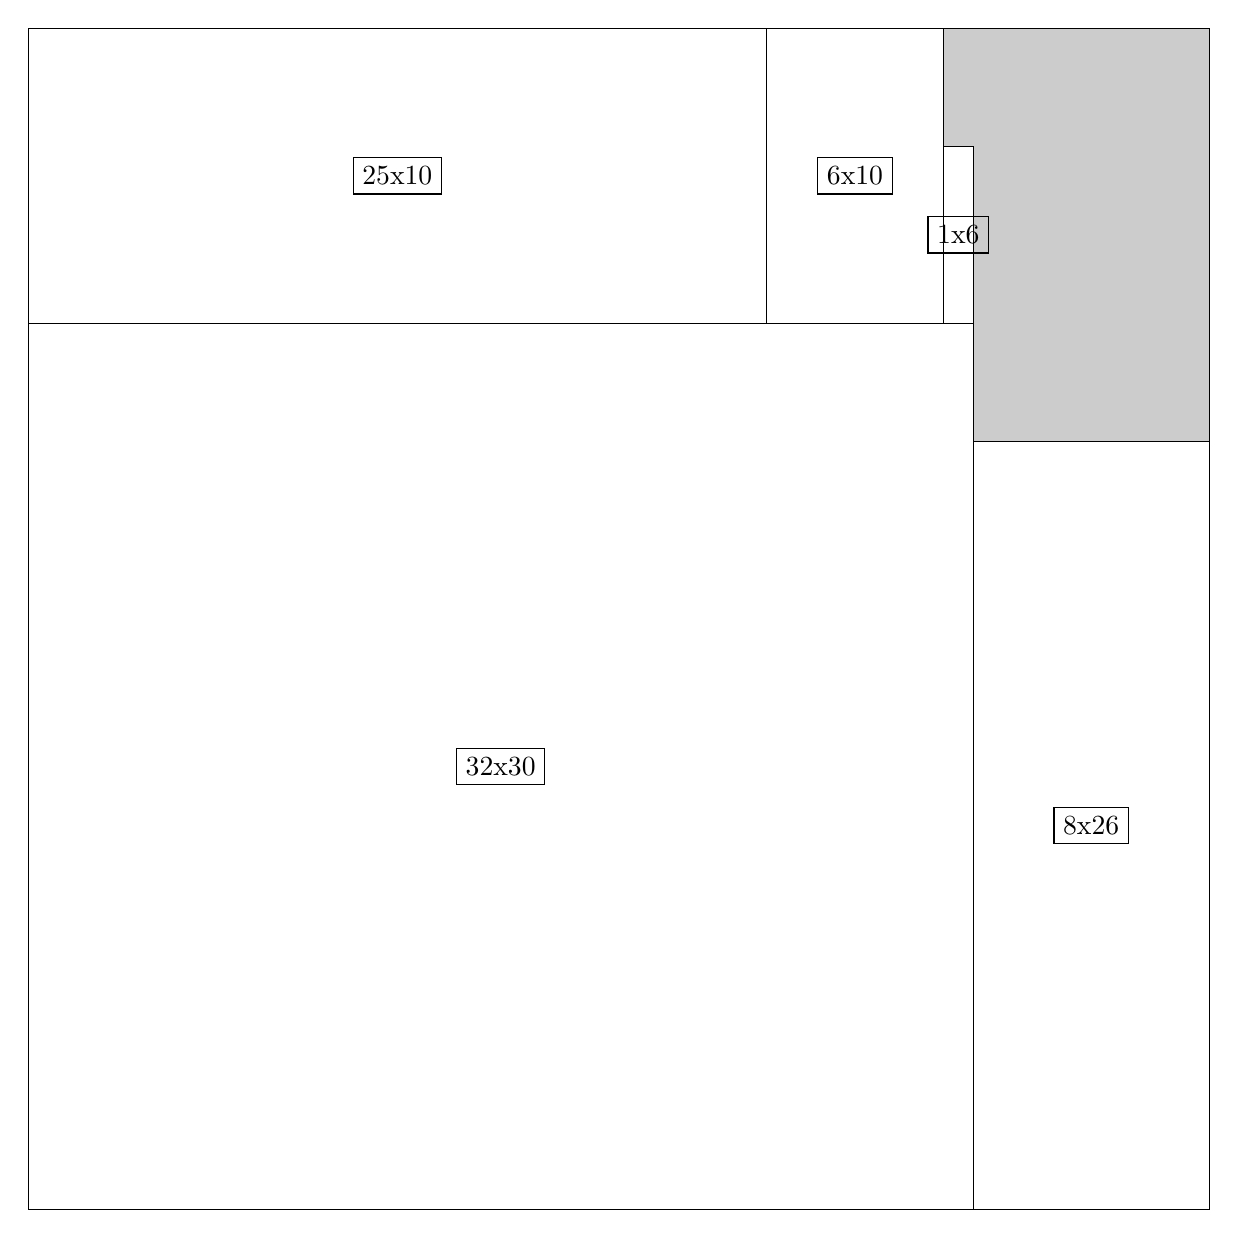
\begin{tikzpicture}[shorten >=1pt,scale=1.0,every node/.style={scale=1.0},->]
\tikzstyle{vertex}=[circle,fill=black!25,minimum size=14pt,inner sep=0pt]
\filldraw[fill=gray!40!white, draw=black] (0,0) rectangle (15.0,15.0);
\foreach \name/\x/\y/\w/\h in {32x30/0.0/0.0/12.0/11.25,25x10/0.0/11.25/9.375/3.75,8x26/12.0/0.0/3.0/9.75,6x10/9.375/11.25/2.25/3.75,1x6/11.625/11.25/0.375/2.25}
\filldraw[fill=white!40!white, draw=black] (\x,\y) rectangle node[draw] (\name) {\name} ++(\w,\h);
\end{tikzpicture}


w =32 , h =30 , x =0 , y =0 , v =960
\par
w =25 , h =10 , x =0 , y =30 , v =250
\par
w =8 , h =26 , x =32 , y =0 , v =208
\par
w =6 , h =10 , x =25 , y =30 , v =60
\par
w =1 , h =6 , x =31 , y =30 , v =6
\par
\newpage


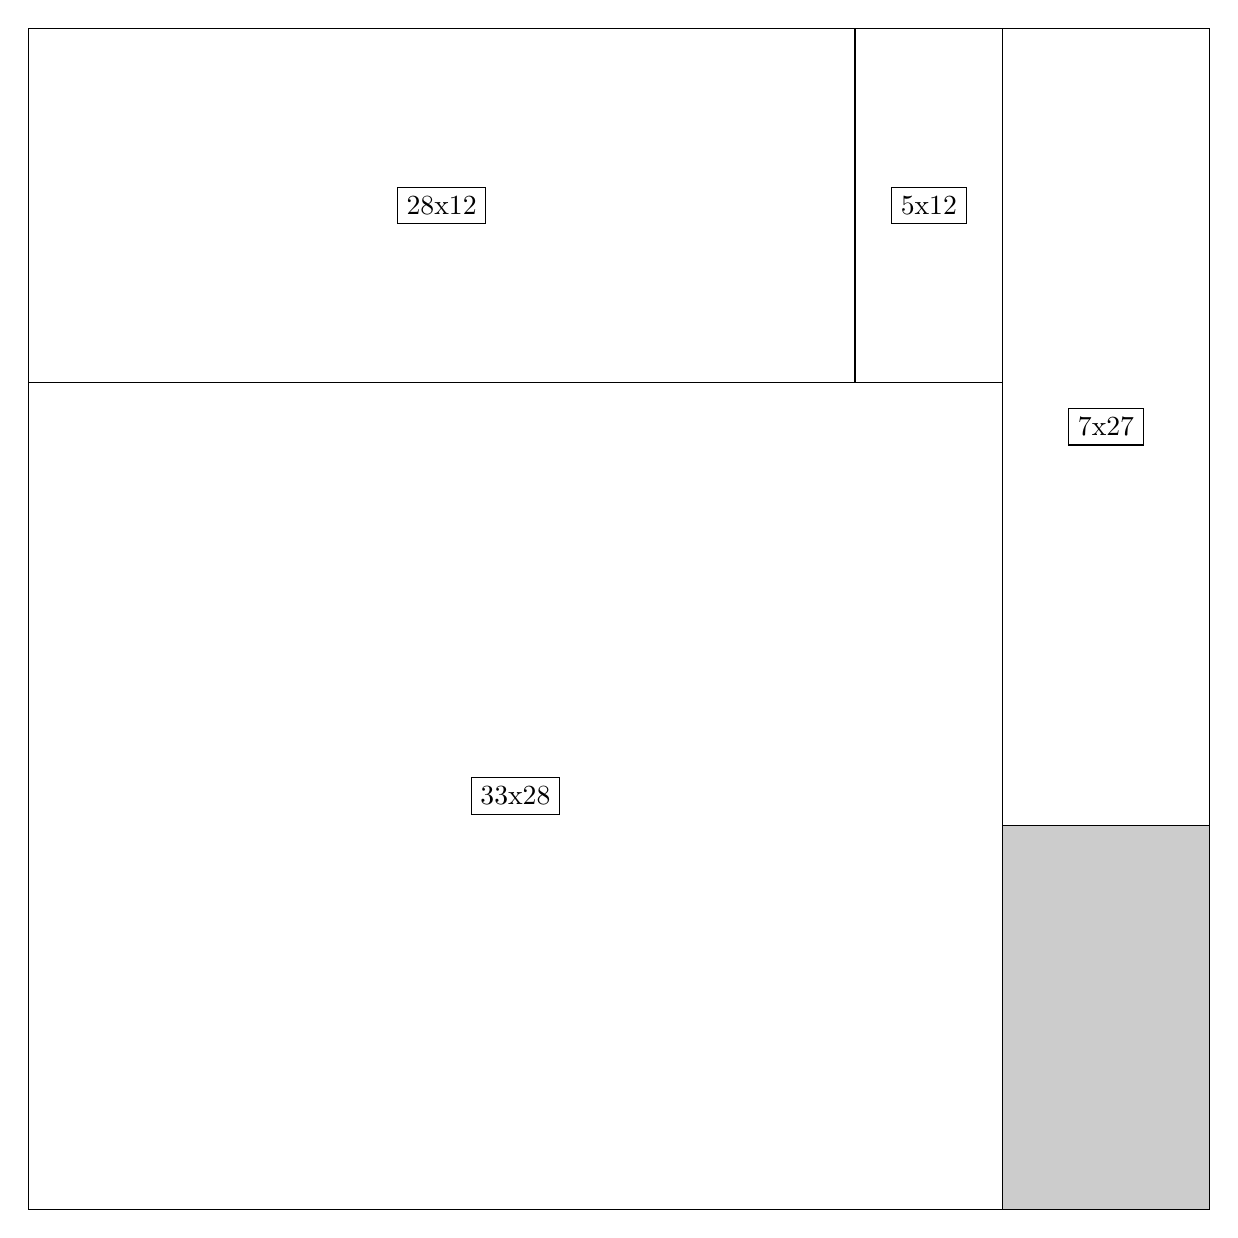
\begin{tikzpicture}[shorten >=1pt,scale=1.0,every node/.style={scale=1.0},->]
\tikzstyle{vertex}=[circle,fill=black!25,minimum size=14pt,inner sep=0pt]
\filldraw[fill=gray!40!white, draw=black] (0,0) rectangle (15.0,15.0);
\foreach \name/\x/\y/\w/\h in {33x28/0.0/0.0/12.375/10.5,28x12/0.0/10.5/10.5/4.5,7x27/12.375/4.875/2.625/10.125,5x12/10.5/10.5/1.875/4.5}
\filldraw[fill=white!40!white, draw=black] (\x,\y) rectangle node[draw] (\name) {\name} ++(\w,\h);
\end{tikzpicture}


w =33 , h =28 , x =0 , y =0 , v =924
\par
w =28 , h =12 , x =0 , y =28 , v =336
\par
w =7 , h =27 , x =33 , y =13 , v =189
\par
w =5 , h =12 , x =28 , y =28 , v =60
\par
\newpage


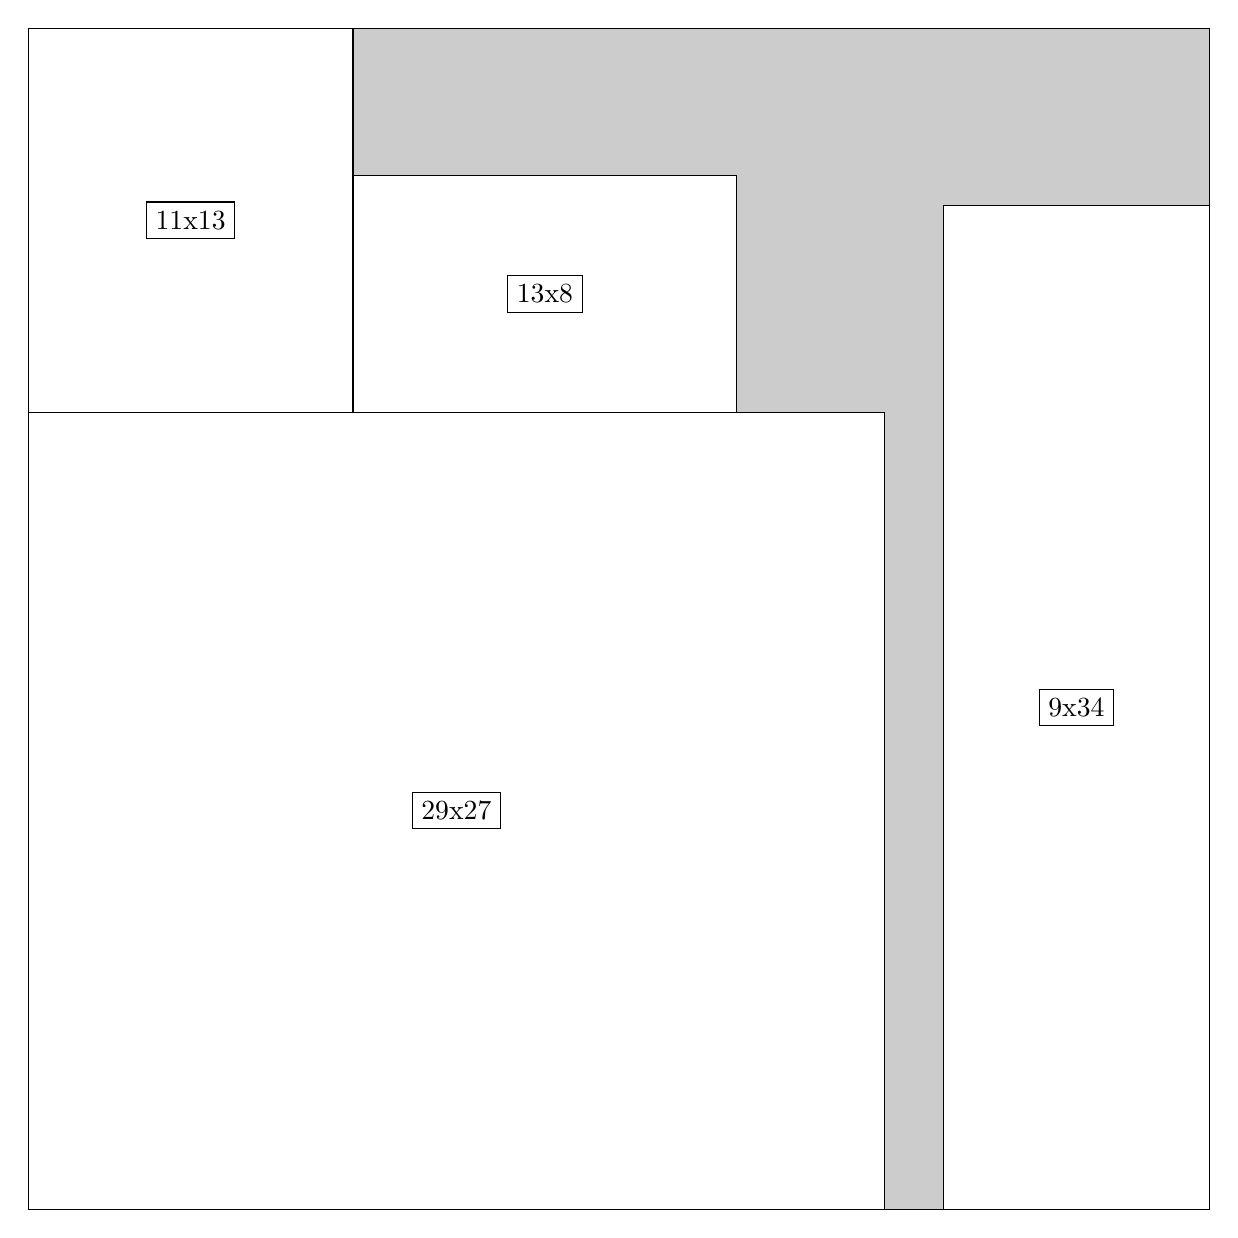
\begin{tikzpicture}[shorten >=1pt,scale=1.0,every node/.style={scale=1.0},->]
\tikzstyle{vertex}=[circle,fill=black!25,minimum size=14pt,inner sep=0pt]
\filldraw[fill=gray!40!white, draw=black] (0,0) rectangle (15.0,15.0);
\foreach \name/\x/\y/\w/\h in {29x27/0.0/0.0/10.875/10.125,9x34/11.625/0.0/3.375/12.75,11x13/0.0/10.125/4.125/4.875,13x8/4.125/10.125/4.875/3.0}
\filldraw[fill=white!40!white, draw=black] (\x,\y) rectangle node[draw] (\name) {\name} ++(\w,\h);
\end{tikzpicture}


w =29 , h =27 , x =0 , y =0 , v =783
\par
w =9 , h =34 , x =31 , y =0 , v =306
\par
w =11 , h =13 , x =0 , y =27 , v =143
\par
w =13 , h =8 , x =11 , y =27 , v =104
\par
\newpage


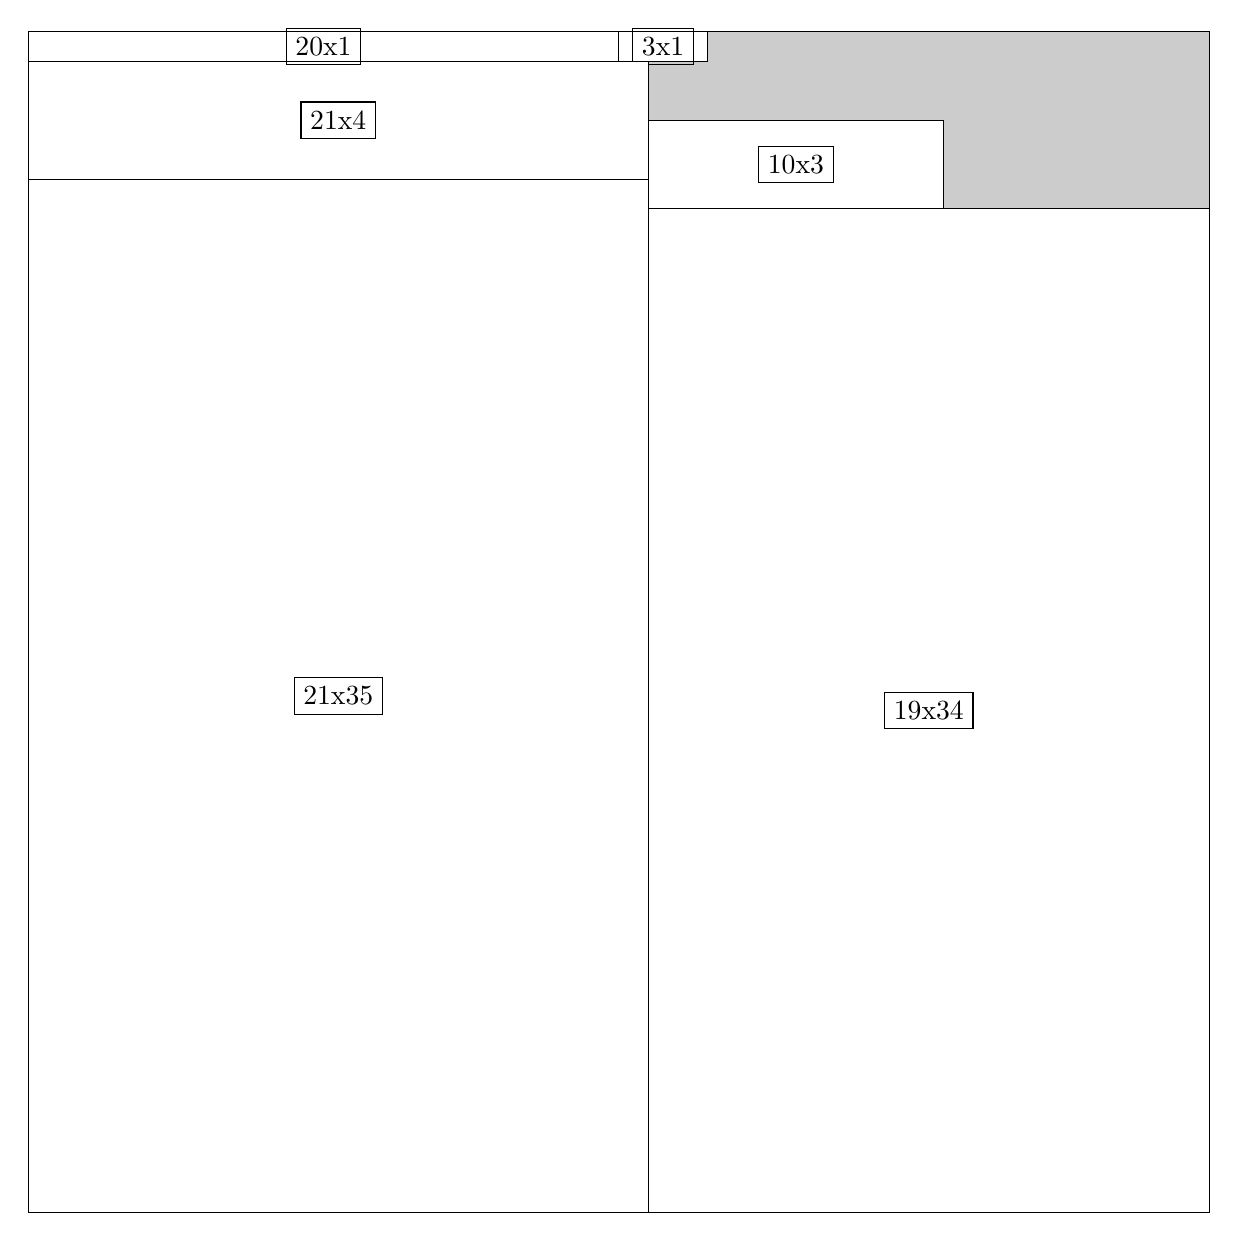
\begin{tikzpicture}[shorten >=1pt,scale=1.0,every node/.style={scale=1.0},->]
\tikzstyle{vertex}=[circle,fill=black!25,minimum size=14pt,inner sep=0pt]
\filldraw[fill=gray!40!white, draw=black] (0,0) rectangle (15.0,15.0);
\foreach \name/\x/\y/\w/\h in {21x35/0.0/0.0/7.875/13.125,3x1/7.5/14.625/1.125/0.375,19x34/7.875/0.0/7.125/12.75,21x4/0.0/13.125/7.875/1.5,10x3/7.875/12.75/3.75/1.125,20x1/0.0/14.625/7.5/0.375}
\filldraw[fill=white!40!white, draw=black] (\x,\y) rectangle node[draw] (\name) {\name} ++(\w,\h);
\end{tikzpicture}


w =21 , h =35 , x =0 , y =0 , v =735
\par
w =3 , h =1 , x =20 , y =39 , v =3
\par
w =19 , h =34 , x =21 , y =0 , v =646
\par
w =21 , h =4 , x =0 , y =35 , v =84
\par
w =10 , h =3 , x =21 , y =34 , v =30
\par
w =20 , h =1 , x =0 , y =39 , v =20
\par
\newpage


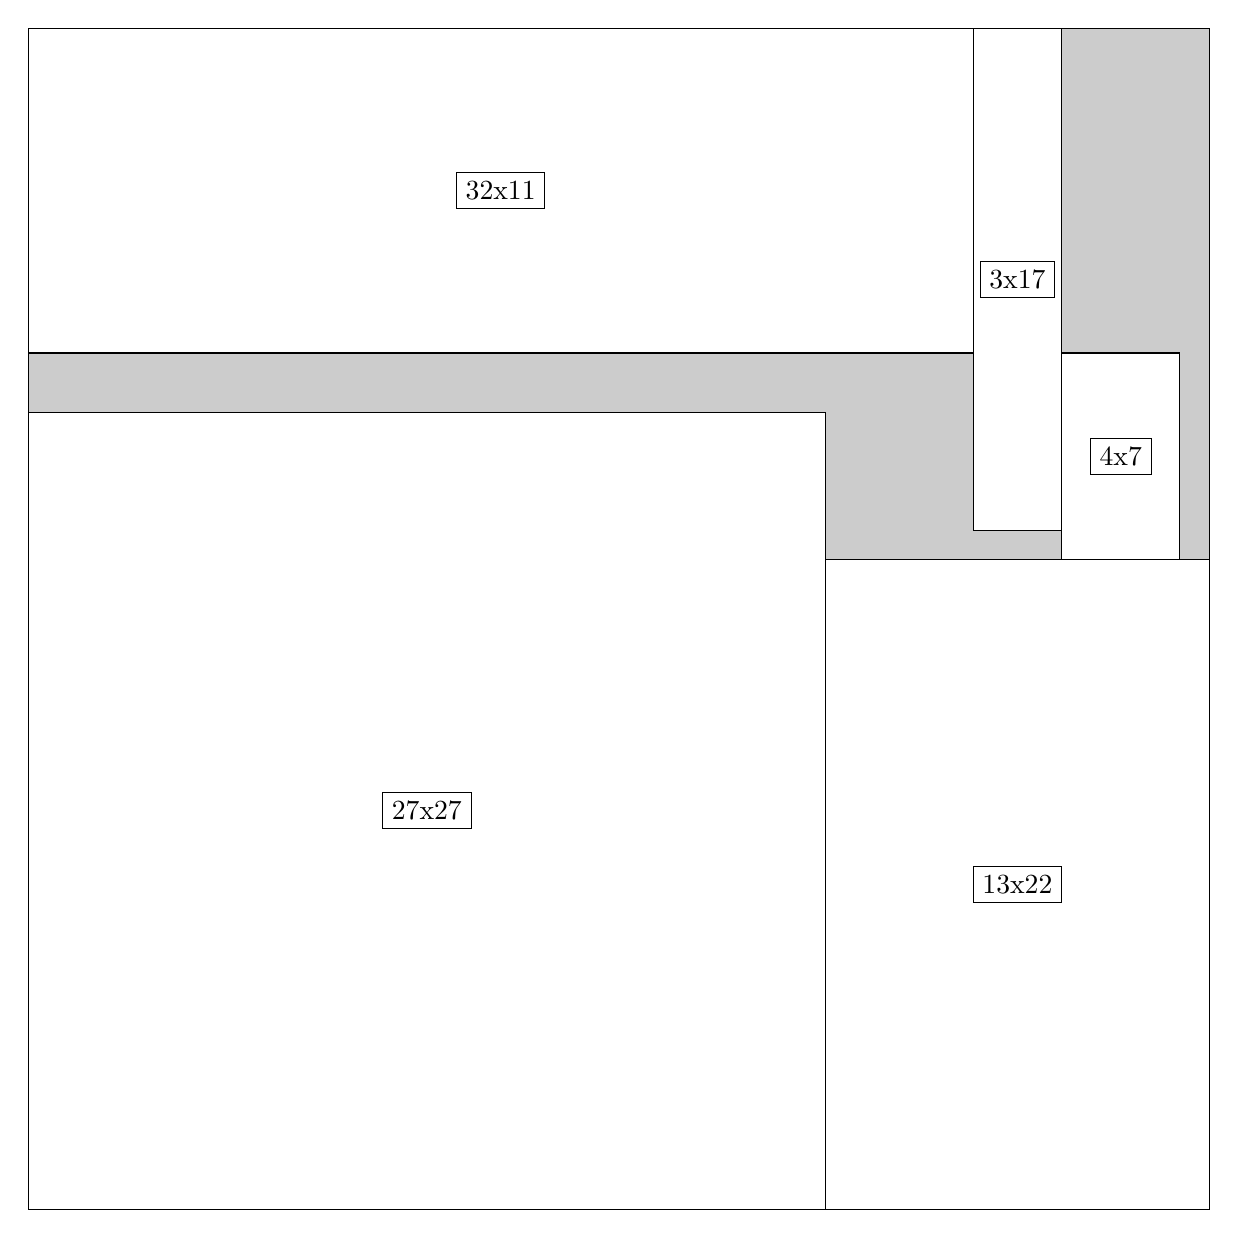
\begin{tikzpicture}[shorten >=1pt,scale=1.0,every node/.style={scale=1.0},->]
\tikzstyle{vertex}=[circle,fill=black!25,minimum size=14pt,inner sep=0pt]
\filldraw[fill=gray!40!white, draw=black] (0,0) rectangle (15.0,15.0);
\foreach \name/\x/\y/\w/\h in {27x27/0.0/0.0/10.125/10.125,32x11/0.0/10.875/12.0/4.125,13x22/10.125/0.0/4.875/8.25,3x17/12.0/8.625/1.125/6.375,4x7/13.125/8.25/1.5/2.625}
\filldraw[fill=white!40!white, draw=black] (\x,\y) rectangle node[draw] (\name) {\name} ++(\w,\h);
\end{tikzpicture}


w =27 , h =27 , x =0 , y =0 , v =729
\par
w =32 , h =11 , x =0 , y =29 , v =352
\par
w =13 , h =22 , x =27 , y =0 , v =286
\par
w =3 , h =17 , x =32 , y =23 , v =51
\par
w =4 , h =7 , x =35 , y =22 , v =28
\par
\newpage


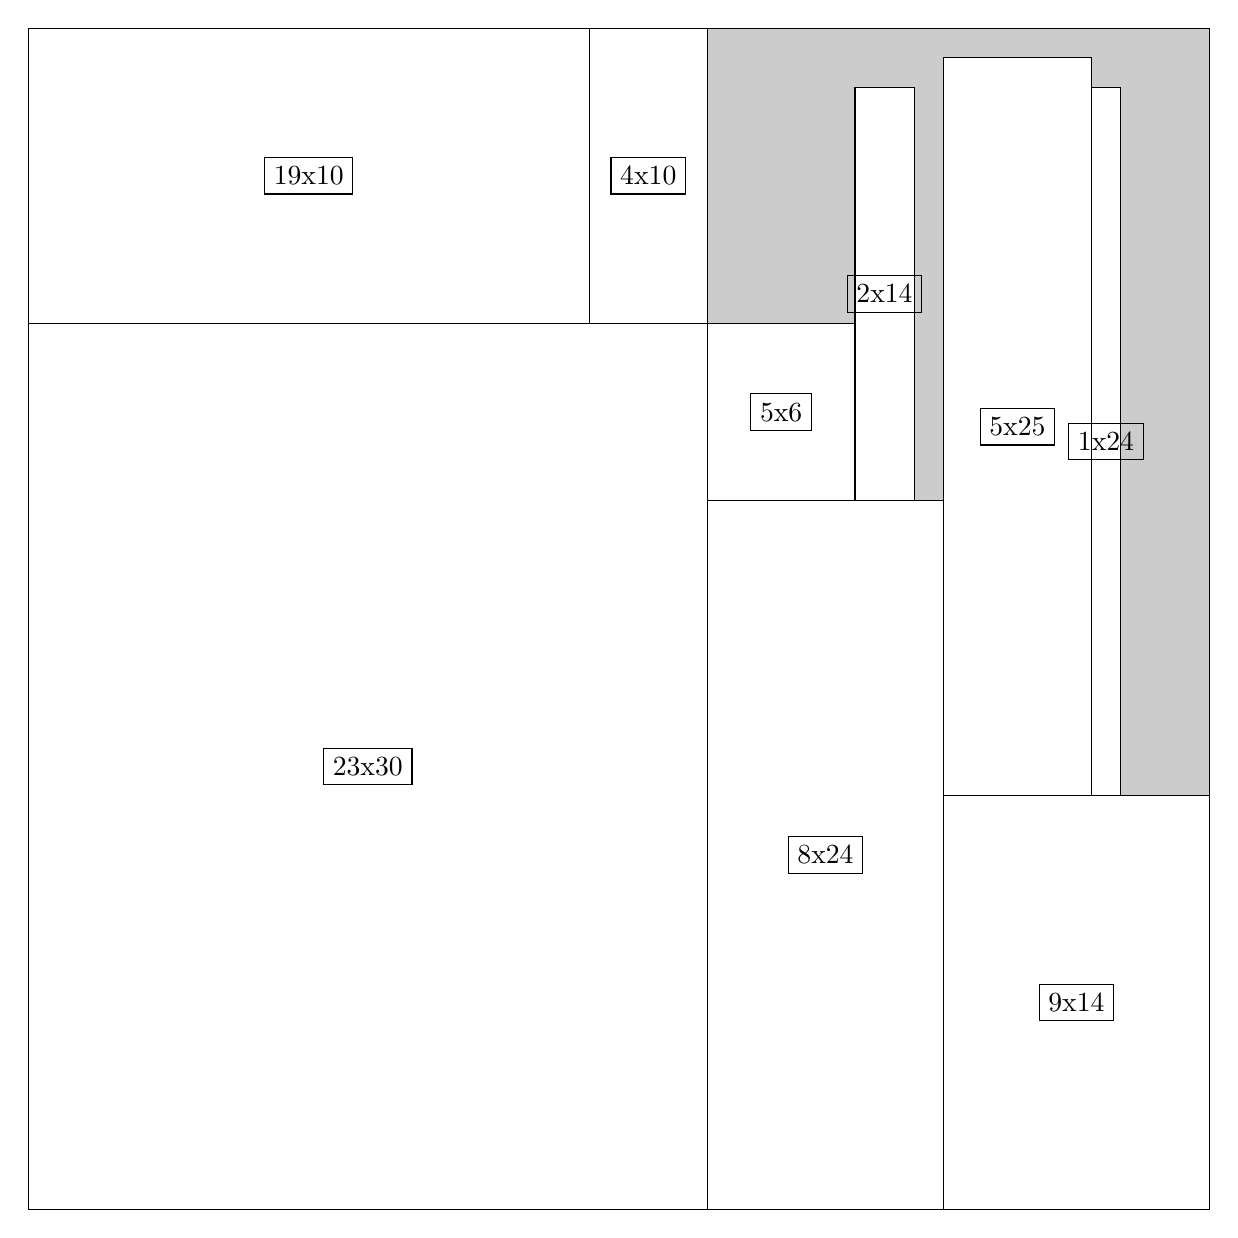
\begin{tikzpicture}[shorten >=1pt,scale=1.0,every node/.style={scale=1.0},->]
\tikzstyle{vertex}=[circle,fill=black!25,minimum size=14pt,inner sep=0pt]
\filldraw[fill=gray!40!white, draw=black] (0,0) rectangle (15.0,15.0);
\foreach \name/\x/\y/\w/\h in {23x30/0.0/0.0/8.625/11.25,8x24/8.625/0.0/3.0/9.0,19x10/0.0/11.25/7.125/3.75,9x14/11.625/0.0/3.375/5.25,5x25/11.625/5.25/1.875/9.375,4x10/7.125/11.25/1.5/3.75,5x6/8.625/9.0/1.875/2.25,2x14/10.5/9.0/0.75/5.25,1x24/13.5/5.25/0.375/9.0}
\filldraw[fill=white!40!white, draw=black] (\x,\y) rectangle node[draw] (\name) {\name} ++(\w,\h);
\end{tikzpicture}


w =23 , h =30 , x =0 , y =0 , v =690
\par
w =8 , h =24 , x =23 , y =0 , v =192
\par
w =19 , h =10 , x =0 , y =30 , v =190
\par
w =9 , h =14 , x =31 , y =0 , v =126
\par
w =5 , h =25 , x =31 , y =14 , v =125
\par
w =4 , h =10 , x =19 , y =30 , v =40
\par
w =5 , h =6 , x =23 , y =24 , v =30
\par
w =2 , h =14 , x =28 , y =24 , v =28
\par
w =1 , h =24 , x =36 , y =14 , v =24
\par
\newpage


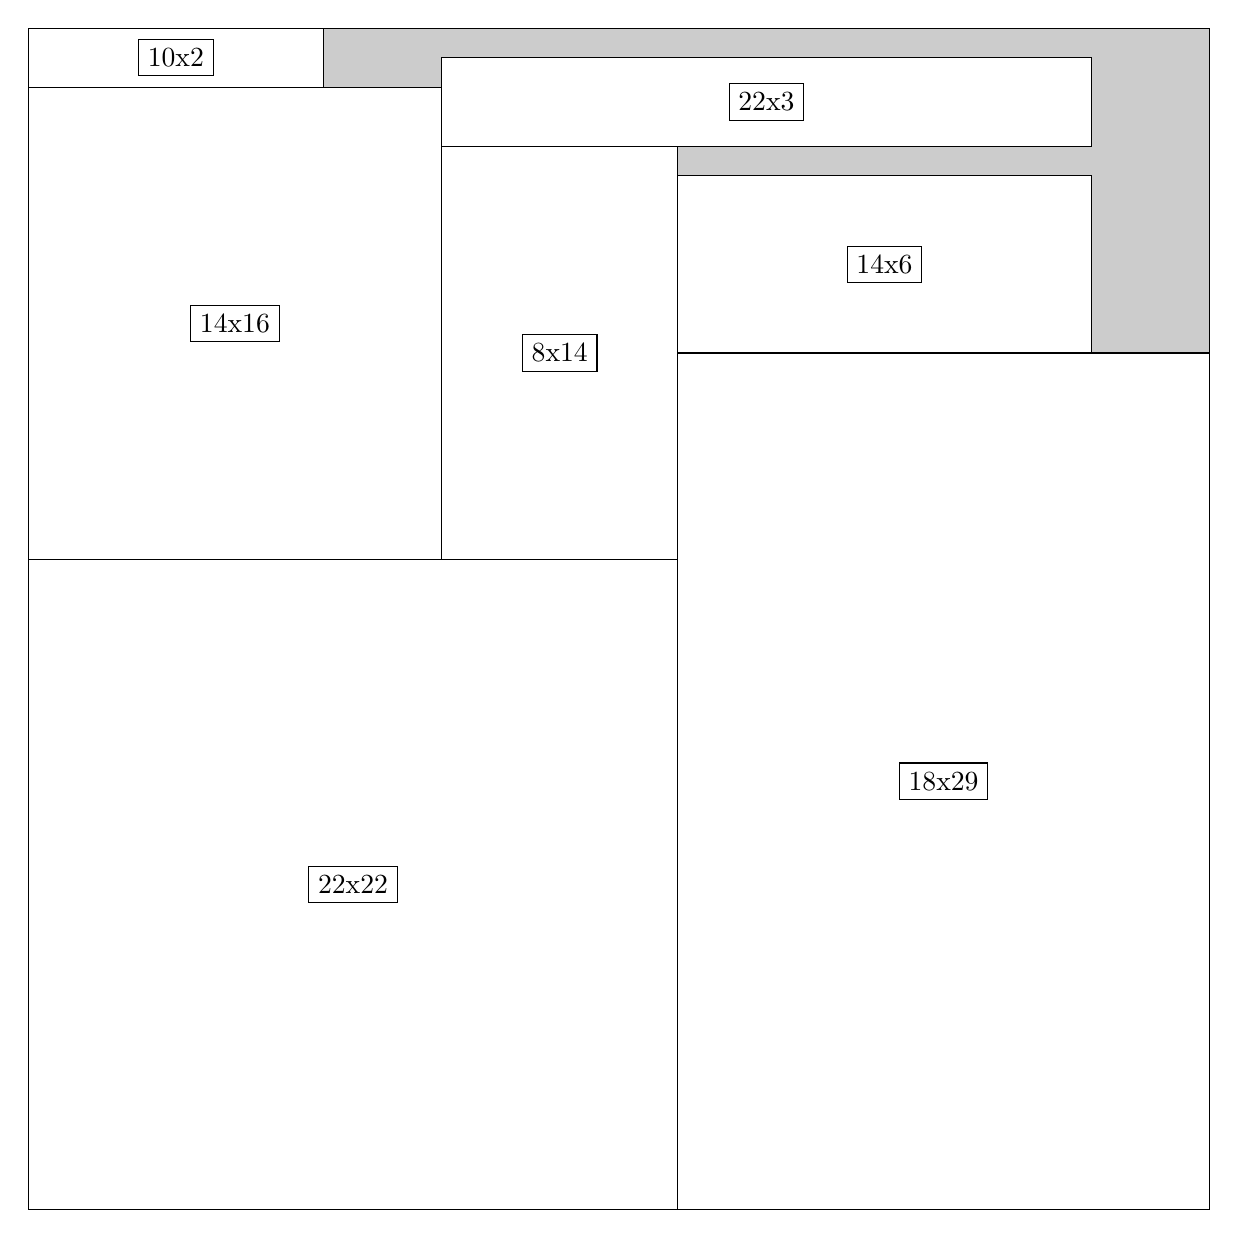
\begin{tikzpicture}[shorten >=1pt,scale=1.0,every node/.style={scale=1.0},->]
\tikzstyle{vertex}=[circle,fill=black!25,minimum size=14pt,inner sep=0pt]
\filldraw[fill=gray!40!white, draw=black] (0,0) rectangle (15.0,15.0);
\foreach \name/\x/\y/\w/\h in {18x29/8.25/0.0/6.75/10.875,22x22/0.0/0.0/8.25/8.25,14x16/0.0/8.25/5.25/6.0,8x14/5.25/8.25/3.0/5.25,14x6/8.25/10.875/5.25/2.25,22x3/5.25/13.5/8.25/1.125,10x2/0.0/14.25/3.75/0.75}
\filldraw[fill=white!40!white, draw=black] (\x,\y) rectangle node[draw] (\name) {\name} ++(\w,\h);
\end{tikzpicture}


w =18 , h =29 , x =22 , y =0 , v =522
\par
w =22 , h =22 , x =0 , y =0 , v =484
\par
w =14 , h =16 , x =0 , y =22 , v =224
\par
w =8 , h =14 , x =14 , y =22 , v =112
\par
w =14 , h =6 , x =22 , y =29 , v =84
\par
w =22 , h =3 , x =14 , y =36 , v =66
\par
w =10 , h =2 , x =0 , y =38 , v =20
\par
\newpage


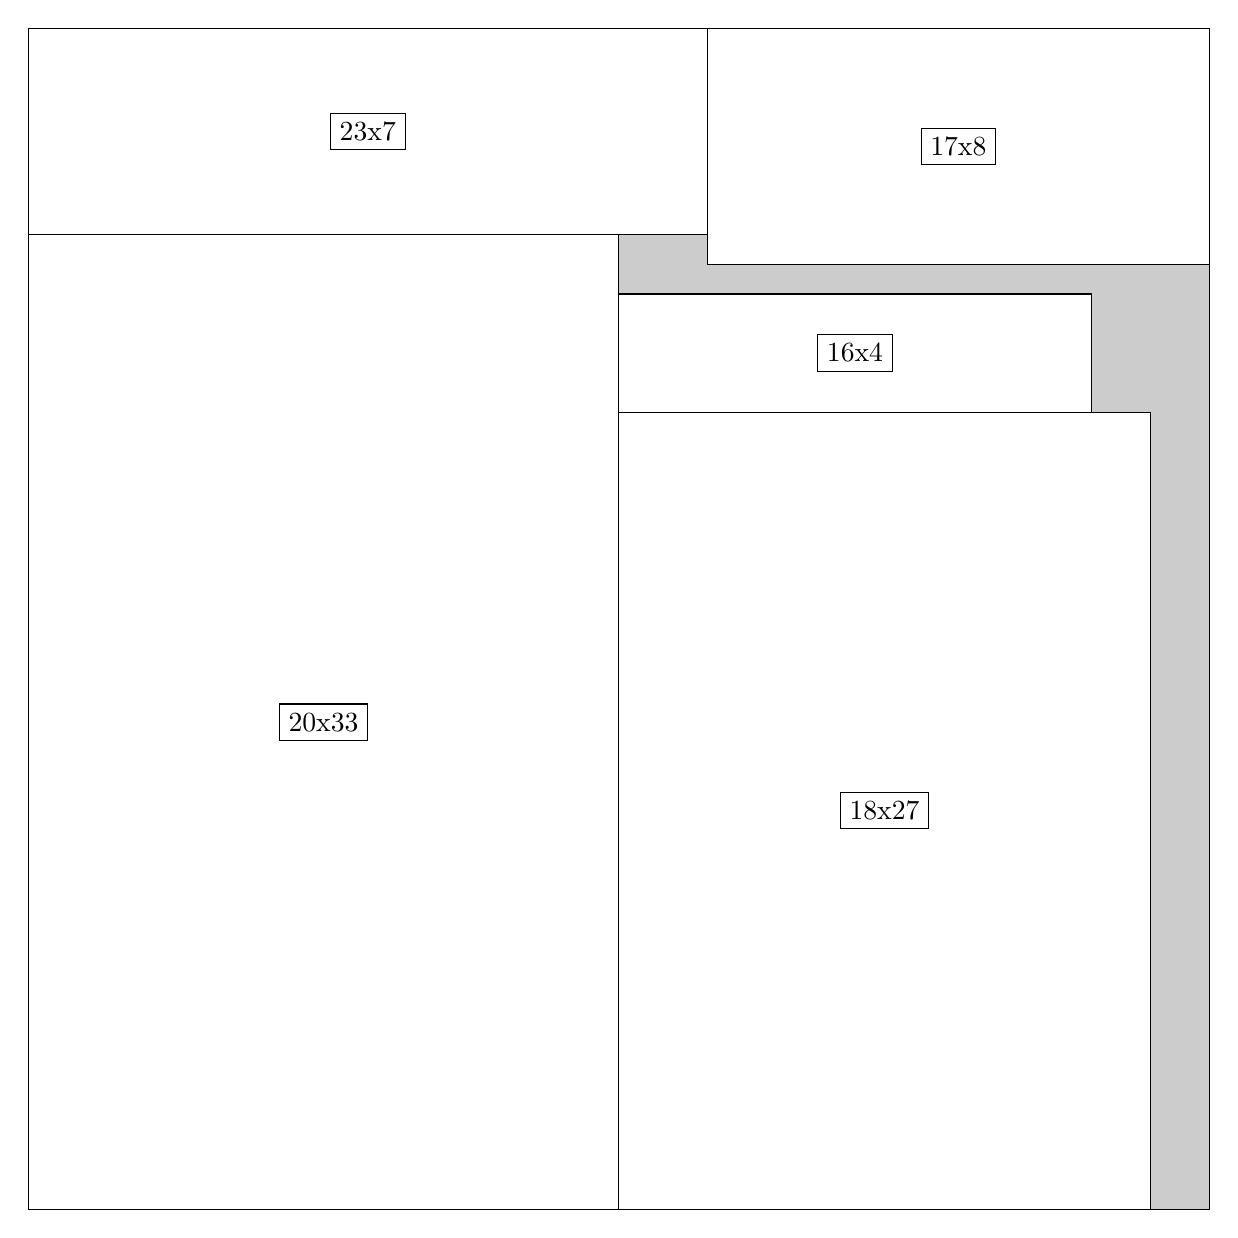
\begin{tikzpicture}[shorten >=1pt,scale=1.0,every node/.style={scale=1.0},->]
\tikzstyle{vertex}=[circle,fill=black!25,minimum size=14pt,inner sep=0pt]
\filldraw[fill=gray!40!white, draw=black] (0,0) rectangle (15.0,15.0);
\foreach \name/\x/\y/\w/\h in {20x33/0.0/0.0/7.5/12.375,18x27/7.5/0.0/6.75/10.125,23x7/0.0/12.375/8.625/2.625,17x8/8.625/12.0/6.375/3.0,16x4/7.5/10.125/6.0/1.5}
\filldraw[fill=white!40!white, draw=black] (\x,\y) rectangle node[draw] (\name) {\name} ++(\w,\h);
\end{tikzpicture}


w =20 , h =33 , x =0 , y =0 , v =660
\par
w =18 , h =27 , x =20 , y =0 , v =486
\par
w =23 , h =7 , x =0 , y =33 , v =161
\par
w =17 , h =8 , x =23 , y =32 , v =136
\par
w =16 , h =4 , x =20 , y =27 , v =64
\par
\newpage


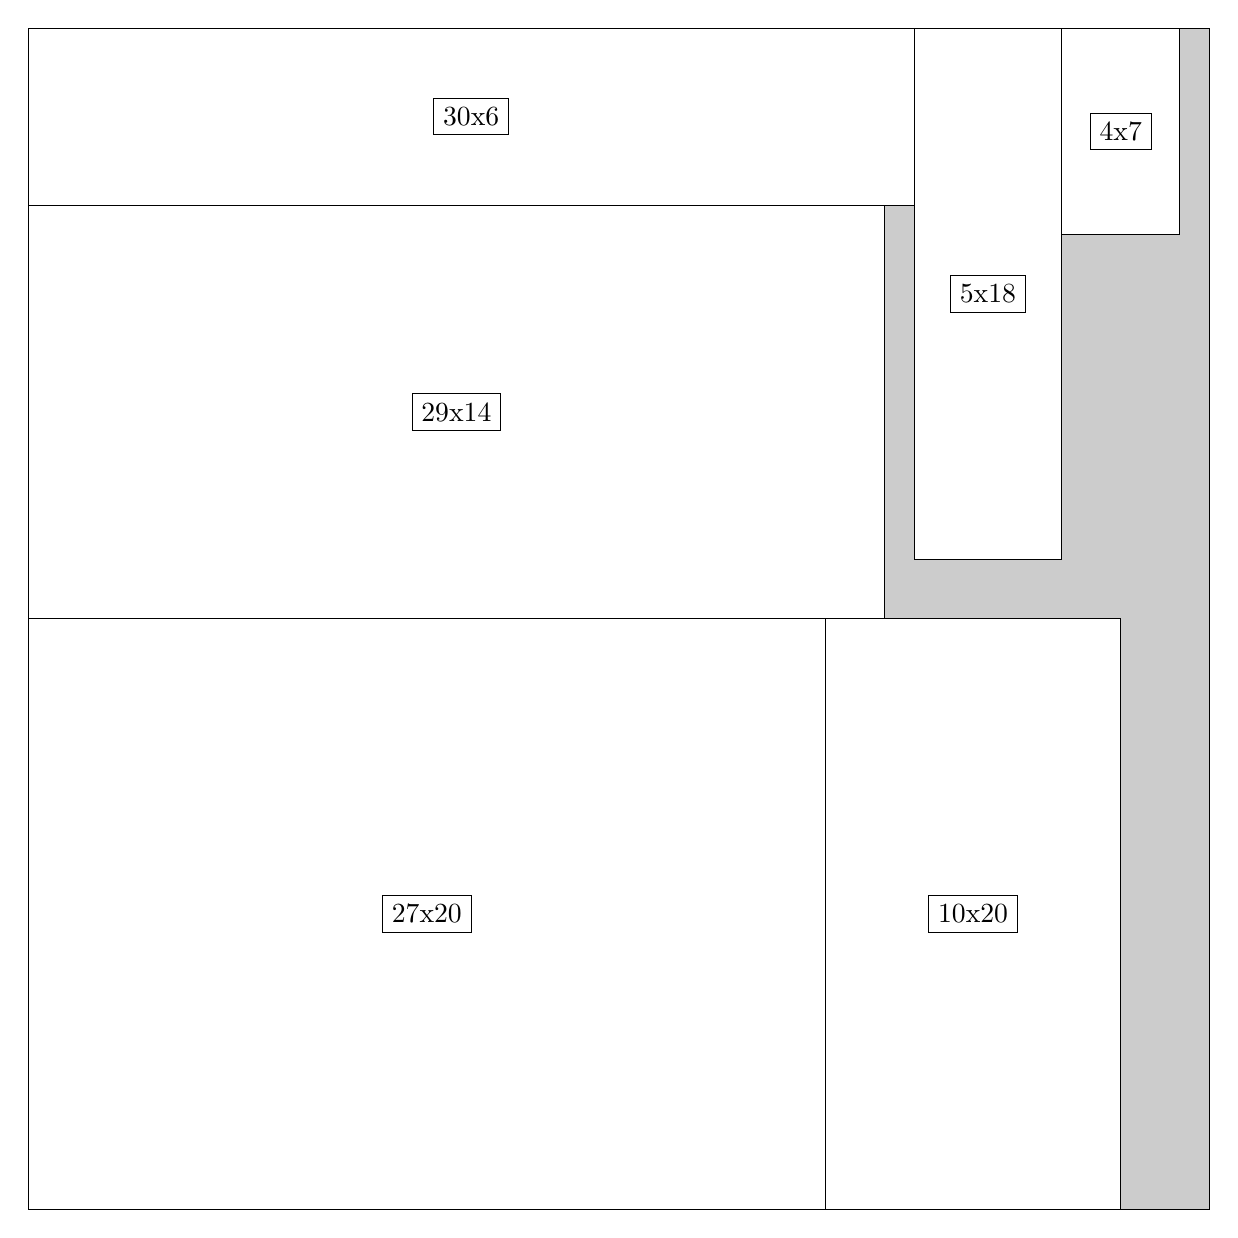
\begin{tikzpicture}[shorten >=1pt,scale=1.0,every node/.style={scale=1.0},->]
\tikzstyle{vertex}=[circle,fill=black!25,minimum size=14pt,inner sep=0pt]
\filldraw[fill=gray!40!white, draw=black] (0,0) rectangle (15.0,15.0);
\foreach \name/\x/\y/\w/\h in {27x20/0.0/0.0/10.125/7.5,29x14/0.0/7.5/10.875/5.25,10x20/10.125/0.0/3.75/7.5,30x6/0.0/12.75/11.25/2.25,5x18/11.25/8.25/1.875/6.75,4x7/13.125/12.375/1.5/2.625}
\filldraw[fill=white!40!white, draw=black] (\x,\y) rectangle node[draw] (\name) {\name} ++(\w,\h);
\end{tikzpicture}


w =27 , h =20 , x =0 , y =0 , v =540
\par
w =29 , h =14 , x =0 , y =20 , v =406
\par
w =10 , h =20 , x =27 , y =0 , v =200
\par
w =30 , h =6 , x =0 , y =34 , v =180
\par
w =5 , h =18 , x =30 , y =22 , v =90
\par
w =4 , h =7 , x =35 , y =33 , v =28
\par
\newpage


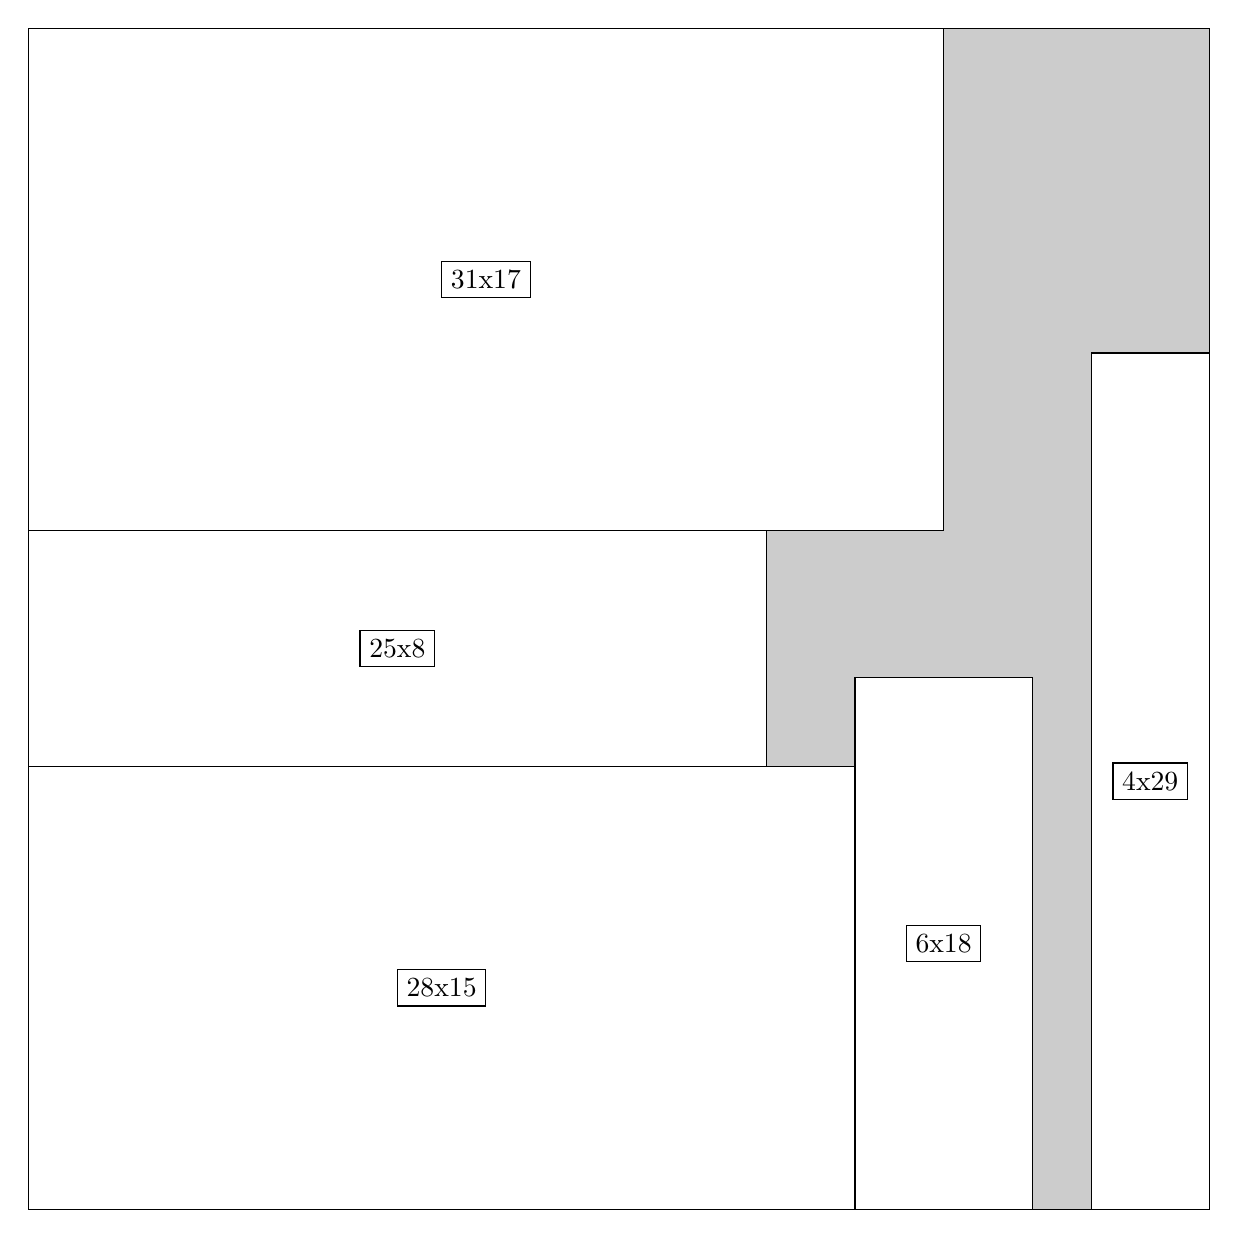
\begin{tikzpicture}[shorten >=1pt,scale=1.0,every node/.style={scale=1.0},->]
\tikzstyle{vertex}=[circle,fill=black!25,minimum size=14pt,inner sep=0pt]
\filldraw[fill=gray!40!white, draw=black] (0,0) rectangle (15.0,15.0);
\foreach \name/\x/\y/\w/\h in {28x15/0.0/0.0/10.5/5.625,31x17/0.0/8.625/11.625/6.375,25x8/0.0/5.625/9.375/3.0,4x29/13.5/0.0/1.5/10.875,6x18/10.5/0.0/2.25/6.75}
\filldraw[fill=white!40!white, draw=black] (\x,\y) rectangle node[draw] (\name) {\name} ++(\w,\h);
\end{tikzpicture}


w =28 , h =15 , x =0 , y =0 , v =420
\par
w =31 , h =17 , x =0 , y =23 , v =527
\par
w =25 , h =8 , x =0 , y =15 , v =200
\par
w =4 , h =29 , x =36 , y =0 , v =116
\par
w =6 , h =18 , x =28 , y =0 , v =108
\par
\newpage


\end{document}